% Don't always start chapter on new page. (http://tex.stackexchange.com/questions/24066/)
\makeatletter
\patchcmd{\chapter}{\if@openright\cleardoublepage\else\clearpage\fi}{\vspace{1in}}{}{}
\makeatother

\nonfrenchspacing

% paper title
% can use linebreaks \\ within to get better formatting as desired
%%%%\title{Making DidFail Succeed \\ 
%%%%Enhancing the CERT Static Taintflow Analyzer for Android App Sets}

% make the title area
%%%%\maketitle
\TODO{emails: (jburket, jlim2, wshen1, wsnavely) @andrew.cmu.edu} \\\wek{Will the students' Andrew email addresses still work after they graduate?  If not, probably best to not include.  Also, don't want to make it too easy for spambots to harvest the email addresses.}
\chapter{Introduction}
\label{sec:intro}
\textit{DidFail} (Droid Intent Data Flow Analysis for Information Leakage) is
static analyzer developed at CERT/SEI that detects possible flows of sensitive
information in sets of Android apps. 
This technical report describes enhancements recently made to the analyzer
itself, a new testing framework, newly developed test apps, and test results. 

The permission system is one of the most crucial features of Android security. By placing adjustable limitations on what resources applications can use, Android allows users to specify in detail how much trust should be given to specific applications. This allows untrusted applications to coexist in an environment with sensitive information, such as the user's location, contacts, and other personal details. 

One of the core assumptions at the heart of the Android permission system is that an application that does not have permission to access a resource has no way in which it can obtain access to that resource. This is enforced with code that checks that an application has permission for a resource when it requests it from the system. Once the application has access to the resource, however, it can use that resource as it sees fit. This can include sharing private information with other applications or executing actions on behalf of another application. Indeed, while the Android permission system is well-suited for controlling access for applications in isolation, it can fail to protect resources, given inter-application communication (ICC).

Consider the case where the user installs an application for recording audio notes. Because the user is recording sensitive information, he or she verifies that the application has no network access. The same user then also installs a weather application, which uses the internet but has access to no sensitive content. Considering the applications in isolation, the user has made sensible decisions: the application which has internet access does not have access to sensitive information and vice versa. If, however, these applications can communicate (either intentionally or unintentionally), then the user's information may still be at risk. If the audio recording application can send messages to the weather app which are then sent over the internet, an outside attacker could gain access to all audio recorded by the device.

As this example demonstrates, the Android permission system alone is insufficient for reasoning about scenarios where information flow between applications circumvents intended permission limitiations. \emph{DidFail}~\cite{didfail} is a tool for detecting such flows. Given a set up of Android APKs, DidFail uses static analysis to detect cases where sensitive information may be leaked from one application to another. While DidFail is a useful tool, it currently falls short in several scenarios. In its previous release, DidFail only tracked flows between Activities via intents. Other types of dataflows, such as those through static fields or between an Activity and a BroadcastReceiver, were previously missed. Through our work, we were able to expand DidFail's capabilities to work with more applications and handle more types of flows (with a few bumps along the way, and some still left for future work). In Sections III-VI, we detail the four features of DidFail we focused on improving.

The DidFail analyzer (source code and binaries), previous DidFail versions, and papers about DidFail are available at: http://www.cert.org/secure-coding/tools/didfail.cfm  The version of DidFail and the test apps described in this report are also directly available at: \TODO{Get URL for direct access and put here, and also populate code, install instructions, and use instructions.}

\chapter{DidFail}

DidFail is a static analysis tool for Android applications that detects possible information flows between applications. DidFail works using two phases: In Phase 1 (Figure~\ref{fig:overview_phase1}), each APK is fed into the \emph{APK Transformer}, a tool that annotates intent-related function calls with extra information that uniquely identifies individual cases where intents are used in the application. Once completed, the transformed APK is passed to two other tools: FlowDroid~\cite{flowdroid} and Epicc~\cite{epicc}.

\begin{figure}[h]
	\centering
	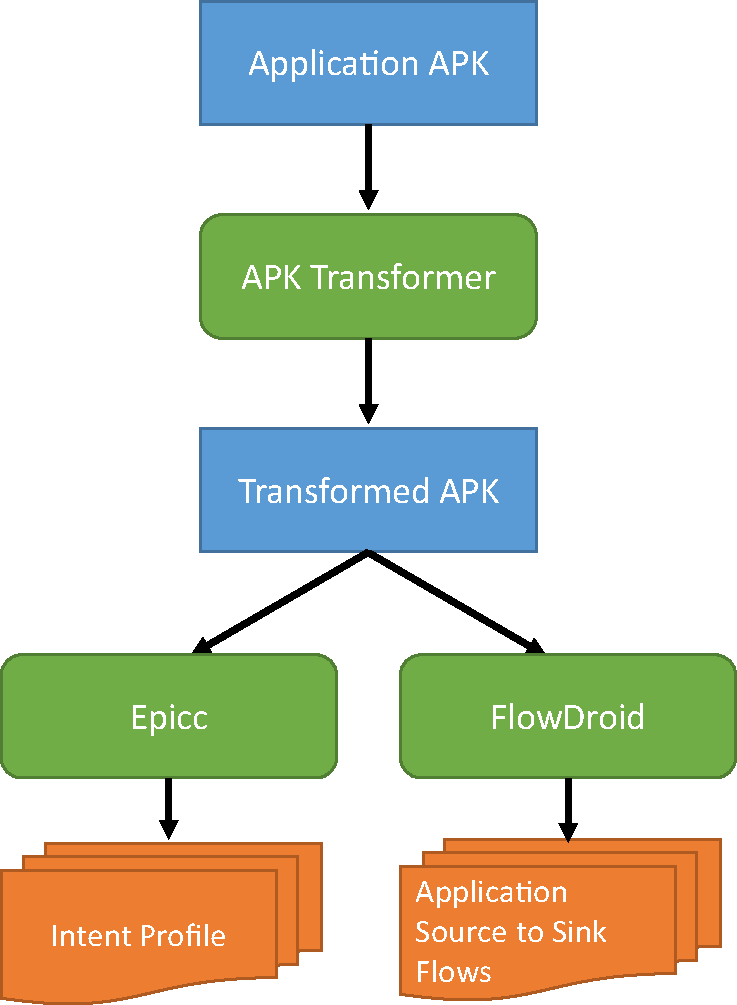
\includegraphics[width=0.35\textwidth]{didfail1.pdf}
	\caption{Overview of DidFail Phase 1}
	\label{fig:overview_phase1}
\end{figure}

FlowDroid is a tool for performing static taint tracking in Android applications. Given a set of method signatures that correspond to taint sources and sinks, FlowDroid conservatively propagates taint from sources in the application, reporting all flows from sensitive sources to sinks. Sinks include function calls that access sensitive information in Android, such as \texttt{getLatitude()} or \texttt{getSimSerialNumber()}. Sinks also include function calls that exfiltrate information, such as \texttt{Log.d} and \texttt{FileOutputStream.write}. In addition, reads from received intents are treated as sources, and writes to intents are treated as sinks. Output from FlowDroid might identify, for example, that an application reads contact information from some source, then sends it as part of an intent, or that an application reads information from an intent, then sends it as an SMS message.

Epicc~\cite{epicc} takes Android applications and performs static analysis to map out inter-component communication within the application. While this is mainly used to understand how parts of a single application work together, it can also discover what portions of the application are externally accessible via either explicit or implicit intents. While FlowDroid is useful for understanding flows within an application, Epicc reveals the interfaces that can be used for an application to communicate with other applications.

Phase 1 of DidFail can be performed on one application at a time and, once completed, does not need to be run again. Phase 2 of FlowDroid combines the Phase 1 output of multiple applications to determine how specific applications in a set can interact. Consider our example from Section~\ref{sec:intro} of the audio and the weather applications. If these applications colluded via an intent, then in Phase 1 DidFail would discover that the audio app obtains audio information (a taint source) and this information flows to an intent sent to an application with a specific name. Similarly, Phase 1 would reveal that the weather app handles intents, reads information from the intent and then sends that information over the internet. 

In Phase 2, DidFail combines the information about these two applications. Realizing that the two applications can communicate via intents, DidFail reasons about dataflows that can occur through intents, eventually discovering and reporting that sensitive audio information is sent over the internet. 

Cases like this one are where DidFail shines. 
Unfortunately, the tool is still limited in the types of flows it can analyze. In our work, we enhanced DidFail to handle more applications and more types of flows.


\chapter{Flows Through Services}
A Service is an application component that is meant to run without direct user interaction (e.g., provide some functionality while the app is not in the foreground). A Service can be instantiated by passing an intent corresponding to a Service's intent filter or the name of the class instance, and making a call to the \emph{startService} method. We added new functionality to DidFail to handle some dataflows involving Services.  

\section{General Modifications}
\subsubsection{Recognizing New Intent Sinks}
DidFail's \emph{APK Transformer} identifies intent sinks in an Android app by matching method signatures in the app with known intent sink method signatures. If the signatures match, an intent ID is generated for the intent sink method. Method signatures for the non-Activity intent sinks were added in order to track intent sinks for BroadcastReceivers and Services. Similarly, FlowDroid had to be modified slightly to recognize the new intent sinks. 

\subsubsection{Matching Flows by Component Types}
DidFail initially only handled flows involving activities. Extending DidFail to also support BroadcastReceiver and Service components required a slight modification in how the sources and sinks were matched. Certain methods indicate the type of a receiving component, and need to be taken into account when matching receiving components and sending components $(e.g.,\  \emph{startService} \rightarrow service, \emph{startActivity} \rightarrow activity).$ By recording the sink component type, we enabled the matching process to create appropriate flows.

\section{Initial Test Results}
We tested the analyzer on a single app set, with two apps that we created. \emph{SendApp}'s main Activity component obtains location information by calling \texttt{getLocation()} and stores the information in an intent set with a custom action string matching \emph{SendAppService}'s intent filter (See Figure~\ref{fig:servicetest1}). The intent is passed to \texttt{startService} and is received by \emph{SendApp}'s Service component, and similarly sent to the \emph{ReceiveAppService} component. \emph{ReceiveAppService} passes the tainted information to \emph{ReceiveApp}'s Activity component by calling \texttt{startActivity}.

\begin{figure}[h]
	\centering
	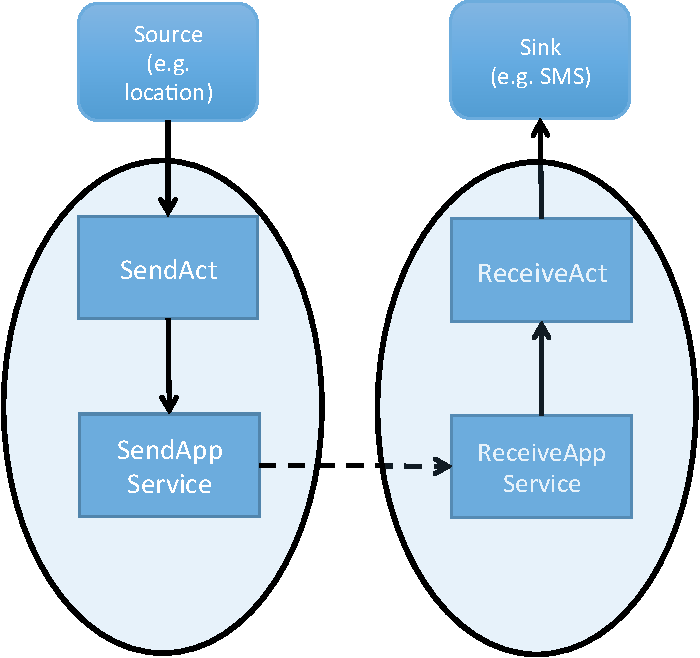
\includegraphics[width=0.35\textwidth]{serviceapp.pdf}
	\caption{Initial App Set for Services}
	\label{fig:servicetest1}
\end{figure}

Phase 1 and Phase 2 analysis results were as expected, tracing the tainted location information through the Activity and Service components, as well as identifying the sources and sinks. We also did a preliminary test run of 100 APKs for Phase 1 using the extended APK Transformer, Epicc and FlowDroid. We observed that intent sinks such as \texttt{startService} and \texttt{bindService} were identified. Further testing still needs to done to verify that the modifications improve Phase 2 results.

\chapter{Incorporating BroadcastReceivers}
The previous version of DidFail did not detect dataflows with broadcast intents. To extend DidFail, we considered aspects of broadcast dataflows. First, broadcast intents are received in a particular way: the app contains a class that extends \texttt{android.content.BroadcastReceiver}, which implements the \texttt{onReceive} method. Second, an application can declare the broadcasts it wishes to receive in two ways: statically in the manifest, or dynamically with the \texttt{registerReceiver()} method. Third, there are different types of broadcasts: normal broadcasts with unordered receivers, ordered broadcasts, and sticky broadcasts that remain active after the initial broadcast distribution is completed.

An app can unregister a dynamically registered receiver (and thereby stop it from receiving broadcasts) by calling the \texttt{Context.unregisterReceiver()} method.  DidFail does not consider calls to \texttt{unregisterReceiver()}; if it can be proven that a receiver cannot be live when a tainted broadcast is sent, then DidFail will produce a false alarm.

We made three modifications to allow DidFail to analyze some dataflows that include broadcast intents. (As mentioned in the Future Work section, a manual kludge is still necessary to handle dynamically registered receivers.) We enhanced the Epicc parser to extract information about broadcast intents, modified FlowDroid to mark broadcast-related functions as sources/sinks, and extended Phase 2 to consume the new output resulting from the previous modifications.

\section{Parsing Epicc Output for BroadcastReceivers}
Dynamically registered receivers do not appear in the manifest, but they do appear in the output of Epicc.  A entry starts with the line ``\texttt{Type:\ android.content.BroadcastReceiver}''.  Potential filter properties are given as a list, e.g., the Actions field in Figure~\ref{fig:bcast_epicc_output} below:

\begin{figure}[!h]
\begin{framed}
\verbatiminput{epicc_br_out.txt}
\caption{Example Epicc Output for a BroadcastReceiver}
\label{fig:bcast_epicc_output}
\end{framed}
\end{figure}

We added a separate parser function named \emph{parse\_bcast} to address this issue. It is used by DidFail in addition to the previously-existing parser function named \emph{epicc\_parser}.

\section{Marking Broadcast Intents as a Sink/Source in FlowDroid}
Function signatures related to transmitting and receiving broadcast intents were added to the APK Transformer and FlowDroid, so that they were recognized as sources/sinks. Table~\ref{fnc_bcast} shows the related functions:
\begin{table}[!h]
\renewcommand{\arraystretch}{1.3}
\caption{Functions Related to Broadcasting Intents}
\label{fnc_bcast}
\centering
\rule{0.55\textwidth}{0.75pt}
\\
\begin{tabular}{l}
%\hline
onReceive \\
sendBroadcast \\
sendBroadcastAsUser \\
sendOrderedBroadcast \\
sendOrderedBroadcastAsUser \\
sendStickyBroadcast \\
sendStickyBroadcastAsUser \\
sendStickyOrderedBroadcast \\
sendStickyOrderedBroadcastAsUser \\
%\hline
\end{tabular}
\\
\rule{0.55\textwidth}{0.75pt}
\end{table}

\section{Trace Broadcast Flows in Phase 2}
The \texttt{taintflows.py} program (the program responsible for executing Phase 2 of DidFail) was extended to parse the additional sink/sources introduced in the previous sections, and do matching of broadcast intent filters. The logic is the same as with non-broadcast intents.

\newpage
\section{Test Applications}
We wrote three toy apps to test this new feature:

\begin{itemize}
\item{} \emph{BroadcastTx} has the READ\_PHONE\_STATE permission and sends the device ID via a broadcast intent with an Action filter. See Figure~\ref{fig:broadcastleak} for the code that leaks the device ID.

\item{} \emph{BroadcastRx\_Static} has the SEND\_SMS permission and receives broadcast intents via a staticly-declared receiver with the same Action filter as declared in the manifest file.  See Figure~\ref{fig:broadcastmanifest} for the manifest, and Figure~\ref{fig:broadcaststaticrecvr} for the receiver class.

\item{} \emph{BroadcastRx\_Dyn} has the ACCESS\_FINE\_LOCATION permission and receives a broadcast intent via a dynamically registered receiver with the same filter.  See Figure~\ref{fig:broadcastregister} for the receiver registration, and Figure~\ref{fig:broadcastdynrecvr} for the receiver class. 
\end{itemize} 

\begin{figure}[!h]
\begin{framed}
\lstinputlisting[language=Java]{java/broadcasttx.java}
\caption{Transmitter code leaking device ID through a broadcast intent}
\label{fig:broadcastleak}
\end{framed}
\end{figure}

\begin{figure}[!h]
\begin{framed}
\lstinputlisting[language=XML]{broadcaststatic.xml}
\caption{Statically declared BroadcastReceiver in a manifest file}
\label{fig:broadcastmanifest}
\end{framed}
\end{figure}

\begin{figure}[!h]
\begin{framed}
\lstinputlisting[language=Java]{java/broadcastonreceive.java}
\caption{Code for a BroadcastReceiver that sends text messages}
\label{fig:broadcaststaticrecvr}
\end{framed}
\end{figure}

\begin{figure}[!h]
\begin{framed}
\lstinputlisting[language=Java]{java/broadcastdyn.java}
\caption{Registering a BroadcastReceiver dynamically}
\label{fig:broadcastregister}
\end{framed}
\end{figure}

\
\begin{figure}[!h]
\begin{framed}
\lstinputlisting[language=Java]{java/broadcastdynrcvr.java}
\caption{Code for a BroadcastReceiver that writes to a file}
\label{fig:broadcastdynrecvr}
\end{framed}
\end{figure}

\section{Results}

Our modified FlowDroid identified the expected sources/sinks in the toy applications. First, it identified the leakage of the device ID through a broadcast intent in Figure~\ref{fig:broadcastleak} as a tainted source. The BroadcastReceivers in Figure~\ref{fig:broadcaststaticrecvr} and Figure~\ref{fig:broadcastdynrecvr} were identified as sinks.

Phase 2 analysis correctly identified two inter-application flows: from the transmitter to the statically registered BroadcastReceiver, and from the transmitter to the dynamically registered BroadcastReceiver.

\section{Future Work}
Currently, for a dynamically registered BroadcastReceiver to be handled by DidFail, a dummy static declaration of the BroadcastReceiver must be added to the manifest file so that FlowDroid can appropriately analyze it. This dummy declaration could be added after analysis of the code shows a BroadcastReceiver is dynamically registered. This problem with analyzing dynamically registered BroadcastReceivers is a known issue of FlowDroid, and we didn't find an easy way to modify FlowDroid to fix this. As future work, we can further investigate how to modify FlowDroid to correct this issue, or alternatively, we can modify the APK Transformer to automatically add this dummy declaration into the app's manifest file.


\newpage
\chapter{Static Field-Based Flows}

There are many ways that two Android applications could potentially communicate with each other. The most direct way is for applications to send and receive intents, which are specifically designed for inter-application communication. Other, more subtle communication mechanisms can also be used to share information between applications, including cooperative use of shared state, or any of a number of covert channels (power usage, timing, etc.). Since DidFail aims to detect how applications can communicate to share permissions, it needs to understand as many of these types of communication channels as possible.

\section{The Issue with Static Fields}

While DidFail is still a ways away from detecting many of these flavors of communication, we were able to successfully add new support for detecting flows through one popular type of shared state: \emph{static shared fields}. A static field in Java (denoted as such using the \texttt{static} keyword) is a field that has one value that is shared among all instances of a specific class. This is used to have state at the class-level rather than the instance-level.

Static fields present an interesting challenge when trying to detect inter-application flows on Android. Consider a hypothetical application \emph{AppChat} that receives intents, appends the contents of received intents to a static String \texttt{chatlog}, and then sends the contents of \texttt{chatlog} back to the application that originally issued the intent. This \emph{AppChat} application allows two applications \emph{A}, \emph{B} to communicate with each other via proxy. \emph{A} can send a message to \emph{AppChat}, that message is saved in the static field \texttt{chatlog}, and then when \emph{B} sends a message to \emph{AppChat} it will receive back the message sent to \emph{AppChat} by \emph{A}. Thus, in an application set containing \emph{A}, \emph{B}, and \emph{AppChat}, we should detect six potential inter-application flows: \emph{A$\rightarrow$AppChat}, \emph{AppChat$\rightarrow$A}, \emph{B$\rightarrow$AppChat}, \emph{AppChat$\rightarrow$B}, \emph{A$\rightarrow$B}, and \emph{B$\rightarrow$A}.

\begin{figure}
\begin{framed}
\lstinputlisting[language=Java]{java/appchat.java}
\caption{Simple Static Field Example}
\label{fig:appchat}
\end{framed}
\end{figure}

Unfortunately, DidFail originally fails to detect some of these potential flows, an issue that has primarily to do with DidFail's use of the FlowDroid tool~\cite{flowdroid}. Recall that FlowDroid takes in an application APK and statically detects potential flows from labeled source and sink functions in that application. In this case, \texttt{getIntent} is considered a source, while \texttt{setResult} is considered a sink. Thus, FlowDroid reports a single flow from \texttt{getIntent} to \texttt{setResult}. Notably, this result is exactly the same as if the static field \texttt{chatlog} had not been used at all (i.e., the received message is simply echoed back as the reply). Indeed, while FlowDroid does track through static fields, it does not indicate their presence in the results. Thus, the second phase of DidFail is unaware of the presence of any static fields in an application.

Given only the flow from \texttt{getIntent} to \texttt{setResult}, DidFail will understand that the \emph{AppChat} application takes in input from an application and then replies to that application based on that input. Thus, DidFail will report the following flows: $I_A\rightarrow R(I_A)$ and $I_B\rightarrow R(I_B)$. These account for four of the six of the flows we described above (\emph{A$\rightarrow$AppChat}, \emph{AppChat$\rightarrow$A}, \emph{B$\rightarrow$AppChat}, \emph{AppChat$\rightarrow$B}). Crucially missing here, however, is the flow between applications \emph{A} and \emph{B}, which can communicate via the static field \texttt{chatlog}. 

\section{Adding Support for Static Field Flows}

In order for DidFail to be able to reason about flows involving static fields, we must modify FlowDroid to report additional information about how static fields are used in an application. Given that static fields serve as a sort of persistent state that can be both read from and written to, it makes sense to treat static fields as if they were both a source \emph{and} a sink. In other words, if sensitive information flows from a source to a static field, we should report this flow, and if content flows from a static field to a sink, we should report this flow as well.

There were a number of key challenges we encountered while trying to add this feature to FlowDroid. First and foremost, FlowDroid only handles sources and sinks that occur as function calls. Thus while it is easy to mark a function as a new taint source, there is no support for adding more general types of sources, such as any read associated with a specific variable. This meant that we needed to modify the actual code associated with FlowDroid's taint analysis in order to achieve our goals.

At a very high level, FlowDroid discovers flows in an application using approximately the following steps:
\begin{enumerate}
\item Load source code of the application, convert this code to Jimple~\cite{soot}, and construct an \emph{exploded supergraph} that models interprocedural interactions. Note here that a node is a statement in Jimple, and an edge is directed, pointing from a node $A$ to $B$ if $B$ could succeed $A$ in some possible program execution. Each node also has some taint status T.
\item Scan through graph and add an edge ($\emptyset$, $N$) for every $N$ that contains a source to a worklist $W$
\item While $W$ is non-empty, pop edge $(N_1, N_2)$ from $W$:
\begin{enumerate}
\item Given the current taint status on $N_1$, run the \emph{flow function} on $(N_1, N_2)$ to produce the current taint status for $N_2$
\item If the taint status of $N_2$ changed, for every child of $N_2$, $N_3$, add edge $(N_2, N_3)$ to the worklist $W$
\end{enumerate}
\item Use the per-statement taint information to compute the source-to-sink flows through the application.
\end{enumerate}

This majority of this algorithm is based on the general IFDS Framework for dataflow analysis~\cite{ifds}. The key component of FlowDroid's instantiation are the \emph{flow functions} used to propagate taint information across edges. These flow functions, of which one is selected based on the type of statement in question, dictate when taint information is created, propagated and destroyed. Consider an assignment statement $x = y$. If $y$ is tainted, then we should mark $x$ as tainted and if $y$ is not tainted, then we do not mark $x$ as tainted. 

Note that in the original FlowDroid, since all taint sources and sinks are function calls, an assignment of the form $x = y$ can only propagate taint, not create or destroy it. In order for us to support static fields, however, we need to change this. We modified the flow function for assignment statements of the form $x = y$ to instead have the following logic:

\begin{itemize}
\item If $y$ is a static field, mark $x$ with taint $T_y$, where $T_y$ is taint originating from static field $y$
\item If $x$ is a static field and $y$ is tainted with taint $T$, add a $T\rightarrow x$ to the list of sink results
\item Otherwise, the taint of $x$ is set to the taint of $y$
\end{itemize}

In addition we altered the original code that seeds the IFDS algorithm with initial edges to also add edges for assignment statements involving reads from static fields. This modification works quite well for basic examples. Considering our example in Figure~\ref{fig:appchat}, FlowDroid would now correctly report the flows $getIntent\rightarrow log$, $log\rightarrow setResult$, and $getIntent\rightarrow setResult$. With the static field information now recorded as extra information flows, we are now in a position to make judgments about inter-application flows through static fields (see Section~\ref{sec:staticphase2}).

\section{Harder Static Field Flows}

\begin{figure}
\begin{framed}
\begin{center}
\begin{minipage}{0.85\textwidth}
\lstinputlisting[language=Java, numbers=left]{java/aliased.java}
\end{minipage}
\end{center}
\caption{Static Fields with Aliasing}
\label{fig:aliased}
\end{framed}
\end{figure}

Unfortunately, this simple solution does not work in any non-trivial case. Consider the situation where a static variable has been \emph{aliased}, as in Figure~\ref{fig:aliased}. In this case, when we run the flow function on the line $\mathit{b2}.x = source()$, we should treat $\mathit{b2}.x$ as a sink since it is a static field. It is not obvious that term $\mathit{b2}.x$ is a static field, however. Indeed it is only the fact that $\mathit{b2}.x$ comes after the line $\mathit{b2} = b$ that causes it to be a static field. What this reveals is that, in the general case, \emph{context is important} for deciding which fields should be treated as static fields. If $\mathit{b2}.x$ occurred after $\mathit{b2} = new Box()$, then we would not consider $\mathit{b2}.x$ to be a sink on Line 8.

Naturally, whether a given term $x.y.z... = t$ is a write to a static field is an undecidable property. We can, however, obtain a conservative guess of which fields are static by creating an additional FlowDroid pass that occurs before the main taint analysis. This pass, which uses the same type of taint analysis, marks all static variables as sources and then propagates taint forward. For the code in Figure~\ref{fig:aliased}, $b$ would be tainted on Line 7, which would cause $\mathit{b2}$ to be tainted. Since $\mathit{b2}$ is tainted, $\mathit{b2}.x$ is also tainted. Once we finish with this initial pass, we record the results of what is tainted in a set.

With this initial pass completed, we now have enough information to solve our aliasing problem. We now no longer need to guess whether $\mathit{b2}.x$ is a static field; we can simply check whether it is in the set of statements marked as tainted in the first pass. With this modification, our flow function for assignment $y = x$ now becomes the following:

\begin{itemize}
\item If $y$ is a static field, mark $x$ with taint $T_x$, where $T_x$ is taint originating from static field $x$
\item If $x$ is a static field \textbf{OR $x$ is in the set of tainted statements from Pass 1}, and $y$ is tainted with taint $T$, add a $T\rightarrow x$ to the list of sink results
\item Otherwise, the taint of $x$ is set to the taint of $y$
\end{itemize}

This reuse of FlowDroid's taint analysis to find static fields turns out to be a pleasant and concise solution. In contrast, our initial attempts at a solution in one pass that involved backtracking were much more complex and did not generalize well.

\section{Phase II Static Field Analysis}
\label{sec:staticphase2}

With Phase I of DidFail now producing information about flows through static fields, we still needed to make use of this information in Phase II. Recall that in our original example involving applications $A$, $B$, and $AppChat$, DidFail found the flows $I_A\rightarrow R(I_A)$ and $I_B\rightarrow R(I_B)$, where $I_A$ and $I_B$ are intents issued by $A$ and $B$, respectively. 

When we run modified FlowDroid on $AppChat$, we obtain the flows $getIntent\rightarrow log$, $log\rightarrow setResult$, and $getIntent\rightarrow setResult$, as mentioned earlier. Since $log$ is a static field that could persist across the handling of multiple intents, we need to give it special treatment. We want it to be the case that \emph{every application} that reads from $log$ is tainted by \emph{every application} that writes to that static field. This effectively amounts to taking the Cartesian product of all reads and writes to the field. We find that application $A$ and $B$ both write to and read from $log$, so taking the Cartesian product we get: $(A, A), (A, B), (B, A), (B, B)$. This result means that in addition to the flow where $A$ and $B$ interact with $AppChat$ in isolation, we must now consider the case where input from $A$ flows to $B$ and vice versa.

These additional flows from the Cartesian product calculation are added to the set of flows before DidFail performs its usual flow matching process (described in detail in the DidFail paper).

\section{Drawbacks, Limitations, and Future Work}

Our analysis appeared to work correctly. While our modifications to support flows through static fields worked quite well in most cases, there are still some issues with our solution. With two taint passes instead of one, our required runtime can be as much as double the runtime of the original analysis. 

More critically, the runtime of FlowDroid also scales with the number of sources, which means that adding a new source for every static field read could also ruin performance depending on how frequently static fields are used. In order to evaluate how important this issue is, we tested 100 APKs that, prior to adding this new feature, were successfully analyzed within the allocated time and memory (using virtual machines with 61 GB and FlowDroid analysis memory allowed to take up to 32 GB) (see Section~\ref{sec:infrastructure}). \TODO{Waiting for Will Snavely to confirm or give different size for FlowDroid runs. \wek{This was confirmed by Will Snavely's email sent on Mon 1/12/2015 at 12:16.}}  Unfortunately, the majority (66 out of 100) now timed out or ran out of heap space. It turns out that most applications use static fields quite frequently, particularly when invoking libraries such as Google Ads. For many of these applications, an additional taint analysis for every static field read was prohibitively expensive. In the future, we will increase virtual machine memory size, to see if that enables successful static field taint analysis of more apps. Virtual machines with 244~GB of memory are available\footnote{http://aws.amazon.com/ec2/pricing/}, which also have 32 virtual cores. Future work will also develop strategies to reduce the number of reads which get traced through the program. 

As noted earlier, detecting which fields are static is undecidable and our taint-based solution is therefore an overapproximation. Thus, some reported flows to static fields may not be realizable in practice. The solution is not a \emph{strict} overapproximation, however, since there are some cases where FlowDroid itself does not recognize that a flow exists at all. We cannot detect flows that use static fields for legitmate flows missed by FlowDroid. 

Finally, our current implementation does not support static fields involving arrays. This should be straightforward to do in future work, however.


\chapter{Infrastructure Improvements}
\label{sec:infrastructure}
The original DidFail implementation experienced a high failure rate in the Phase 1 analysis.  Recall that Phase 1 analysis is run on each APK separately, to find tainted flows therein.  This first step of this analysis involves transforming the input APK, instrumenting the callsite of various intent-sending methods with a unique ID.  This transformed APK is then processed by FlowDroid and Epicc.  With this improvement, we sought to increase the success rate of APK processing in Phase 1.

\section{The Problem}
We identified a few issues that contributed to a high failure rate in Phase 1.  The APK Transformer and FlowDroid rely on the underlying Soot framework to handle reading and writing Android APK files. While the APK Transformer itself rarely failed, FlowDroid often choked on the APK produced by the APK Transformer.  Moreover, some APKs encountered no explicit FlowDroid failures, but were not analyzable in a timely fashion (the FlowDroid invocation ran out of time or memory).   These issues together resulted in a very low success rate in Phase 1.  There were no significant issues encountered with the Epicc tool.  In the time since the original version DidFail was completed in March 2014, a new version of the Soot framework was released, which included significantly better facilities for handling APK files, but it was not completely compatible with code written against the older version of Soot.  A new version of FlowDroid was also released, which used the new version of Soot.

\section{Porting Phase 1}
Our first step was to port the DidFail changes to the latest versions of Soot and FlowDroid.  This involved inspecting the modifications to the old FlowDroid branch, and moving them to the latest FlowDroid branch, then testing for correctness.  Moreover, the APK Transformer was rebased on the latest version of Soot, requiring a few source changes, and further testing.

\section{Measuring Phase 1 Performance}
The next step was to create an instrumented harness for running the various components of Phase 1.  In particular, we were interested in gathering data about FlowDroid, since in previous test runs many APKs timed out during FlowDroid processing.  A small test harness was developed in Python for running various Phase 1 components (the APK Transformer, Epicc, FlowDroid, etc.) with various parameters, and with a specified timeout.  This harness also measured system metrics (e.g., memory usage, CPU usage) while the DidFail analyses were running.  
%\TODO{substitute {\em DidFail analyses} for {\em commands}?} DONE

\section{Initial Testing}
A selection of 90 APKs were chosen randomly from a large set, with the goal of running them through both the old and new versions of DidFail, to evaluate the effectiveness of our changes.  A machine was provisioned from Amazon EC2 to run the test, since it was difficult to secure time on a machine locally with enough resources.  This machine had 4 cores and 32 GB of memory.  FlowDroid was allocated 16 GB of memory (through the heap space parameter to the JVM) and a 15-minute timeout.  APKs were processed by the APK Transformer before being sent to FlowDroid.  The graph in Figure~\ref{fig:initial_phase1} summarizes the results of this test.

\begin{figure}[h]
	\centering
	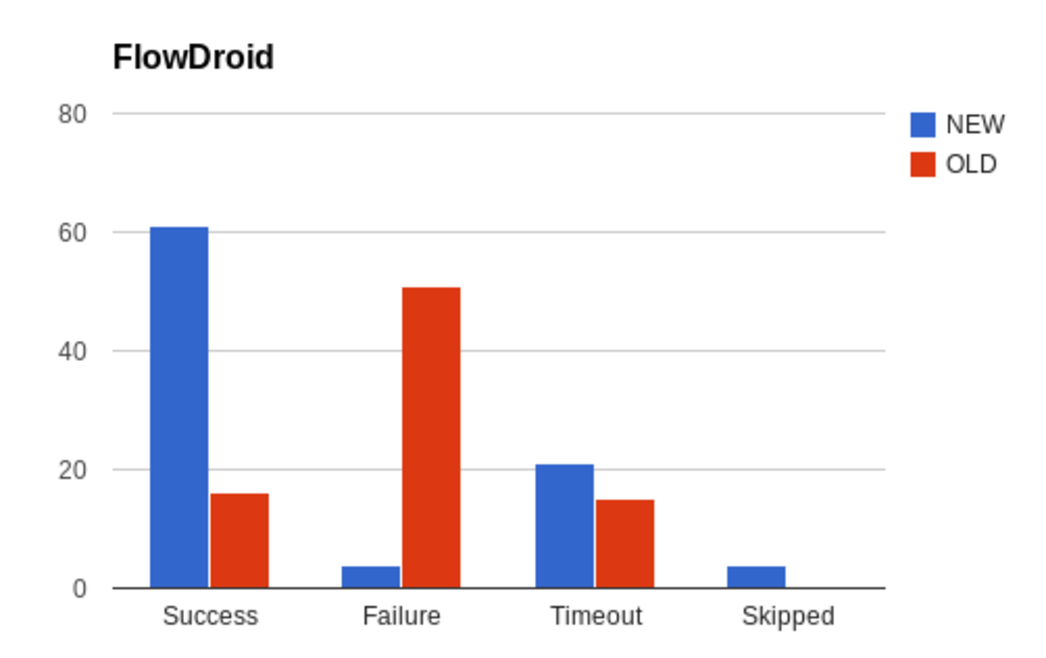
\includegraphics[width=0.50\textwidth]{flowdroid_success.pdf}
	\caption{Results of Flowdroid test run, with and without modifications}
	\label{fig:initial_phase1}
\end{figure}

We see that the number of APKs successfully processed by FlowDroid roughly tripled.   Very few failures were experienced.  A few APKs were skipped due to errors in the transformation stage.  21 of the APKs timed out during FlowDroid analysis, 5 more than timed out in the initial run.  The smaller number of timeouts in the initial run may be explained by the high failure rate: if more APKs hadn't run into runtime exceptions, they may have eventually timed out.  This test run showed that our modifications substantially improved the baseline success rate of Phase 1 analysis.

\section{FlowDroid Performance Tweaks}
Next, we investigated the 21 timeouts in the FlowDroid test.  By reviewing the performance counters, we saw that these analyses consumed all the memory allocated to them (16GB), and were unable to make further progress.

The first thing we tried was vertical scaling.  We provisioned a much larger machine, and re-ran FlowDroid on one of the timed-out APKs.  This was not productive.  Despite allocating nearly 170GB of memory to the process, and disabling timeouts, the analysis reached the same state as before: consuming all allocated memory, and making next-to-no progress forward.  Here is a graph of memory usage over time (approximately 2 hours) for that analysis attempt:

\begin{figure}[h]
	\centering
	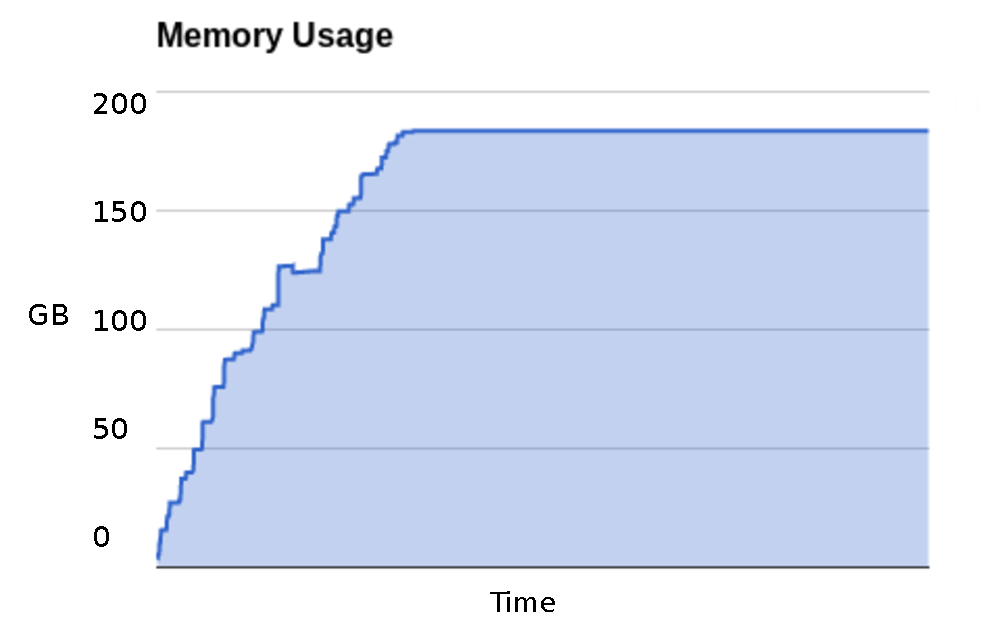
\includegraphics[width=0.50\textwidth]{flowdroid_perf.pdf}
	\caption{Results of FlowDroid test run on high performance machine}
	\label{fig:high_phase1}
\end{figure}

It was clear that the analysis itself needed tuning.  Recall that FlowDroid seeks to construct paths between sources and sinks in an application.  Thus, two fundamental aspects we can tweak are the source/sink identification process and the pathfinding process.  Regarding the former, we can try to reduce the number of sources and sinks by filtering them in some fashion.  Regarding the latter, we can reduce the precision of the pathfinding process.  Of course, this impacts the quality of the analysis.  Filtering the sources/sinks may cause FlowDroid to miss a potentially dangerous flow.  Dumbing down the pathfinding bears this risk as well, and carries the additional risk of introducing false positives. 

Nonetheless, we were interested to determine how much tuning FlowDroid required in order to process the remaining 21 APKs.  We provisioned the same machine as before (32 GB of memory, 4 cores), and maintained the same timeout (15 minutes).  

We first tried source/sink filtering, using the FlowDroid parameters \texttt{nocallbacks} and \texttt{layoutmode}.  The first disables the emulation of Android callbacks (due to button clicks, GPS location changes, etcetera), while the second ignores Android GUI components, like input fields, as data flow sources.  With this change, 9 out of the 21 APKs now were successfully processed by FlowDroid. 

Next, we tuned the pathfinding precision by setting the \texttt{aplength} parameter.  This parameter accepts an integer, and sets the FlowDroid \emph{access path} length.  Consider an expression like \texttt{X.Y.Z = 5}.  Z has an access path length of 2.  Through this parameter, one can configure how deeply FlowDroid will search access paths when tracking taint.  In previous test runs, we had set the path length to 1, so for this tuned run we tried setting the path length to 0.  Six of the twelve remaining APKs now succeeded. 

The final, rather drastic option is the \texttt{nopaths} parameter, which causes FlowDroid to invest no effort in constructing accurate paths.  Rather, it will simply report source/sink pairs.  Obviously, this is bound to produce many false positives.  Nonetheless, this option was required for the remaining six APKs to make it through FlowDroid without timing out.
\section{Conclusions and Future Work on Infrastructure Improvements}
With this work, we substantially improved the success rate of Phase 1 analysis, and investigated the performance of FlowDroid.  We found that vertical scaling is not a viable solution, in many cases, to FlowDroid timeouts.  Moreover, we found that some APKs will not yield to (timely) FlowDroid analysis without very liberal compromises on path precision.

There are two broad directions for future work.  First, more effort can be invested into Phase 1.  FlowDroid, perhaps, could be made to be more resource efficient.  Also, more configuration options could be added to FlowDroid, to allow more granular tuning of the pathfinding process.  Further, the results reported here do not include the modifications made as part of the rest of the project (initial enhancements for analysis of dataflows which traverse shared static fields, Service components, and BroadcastReceiver components).  These additions increase the work required by the Phase 1 analysis, in some cases non-trivially.  At the time of writing, we have preliminary results that show increased timeouts when FlowDroid is run with these additions, using the same hardware configuration.  In summary, building a Phase 1 analysis that accurately finds a wide variety of flows, in a timely fashion, is a difficult problem, one that requires a variety of compromises. 

Next, Phase 2 analysis needs some attention.  Some interesting questions include: How does tuning down the precision of Phase 1 affect Phase 2 results?  Now that more APKs can be processed by Phase 1, can we find legitimate, inter-applications flows in the wild with Phase 2 analysis?

\chapter{Related Work}
\cite{li2015icse} \TODO{Write about IccTA, Adrienne Porter Felt's permissions papers (2), SuSI, others}

\chapter{Conclusions and Future Work}

In our work, we made four improvements to DidFail to help it succeed with more applications and detect more flows. 
 The new setup for instrumented cloud-based testing enables us to take advantage of Amazon's powerful virtual machines and to use virtual machines in parallel for faster test completion. We will continue to use the instrumentation in the new setup, to monitor and optimize DidFail's performance. DidFail was modified to use the most current version of FlowDroid and Soot, and the new version of DidFail was able to successfully process three times as many apps as it was able to previously. The enhancements discussed in this paper moved us significantly closer to the goal of analyzing taint flows through all types of components and shared static fields.
There are still more dataflows that need to be detected and analyzed, but our work has helped improve DidFail as a practical security tool. As future work, we will ensure that dynamically registered BroadcastReceivers can be automatically analyzed by DidFail.
 With a few more improvements, we hope that DidFail can ultimately be incorporated as part of a review process for vetting applications for malicious behavior.
%There are still more flow types that need to be detected (such as flows through the file system, arrays of shared static fields, ordered broadcasts, and sticky broadcasts), but our work has helped improve DidFail as a practical security tool. With a few more improvements, we hope that DidFail can ultimately be incorporated as part of a review process for vetting applications for malicious behavior.


%\bibliographystyle{IEEEtran}
\bibliographystyle{plain2}
\bibliography{content/bib,content/bibliography}

\end{document}
